%=============================================================================
% RAPPORT PFE — Maintenance Prédictive des Roulements Industriels
% Auteur : Mohamed Yassine Balti — ISG Bizerte / Novation City
% Version corrigée : conforme au code source réel (août 2026)
% Sources de vérité utilisées pour cette révision :
%   - models/metrics_v3.csv       (métriques officielles du modèle V7 déployé)
%   - models/metrics_rul_v1.json  (métriques du modèle RUL GradientBoostingRegressor)
%   - README.md                   (architecture, endpoints, historique des corrections)
%   - api_unified_pythagore.py, auth.py, alert_manager.py, reporting_module.py
%=============================================================================

\documentclass[12pt,a4paper]{report}

% ── Encodage et langue ────────────────────────────────────────────────────────
\usepackage[utf8]{inputenc}
\usepackage[T1]{fontenc}
\usepackage[french]{babel}

% ── Mise en page ──────────────────────────────────────────────────────────────
\usepackage[top=2.5cm,bottom=2.5cm,left=3cm,right=2.5cm]{geometry}
\usepackage{setspace}
\onehalfspacing

% ── Graphiques et couleurs ────────────────────────────────────────────────────
\usepackage{graphicx}
\usepackage[table,xcdraw]{xcolor}
\usepackage{tikz}
\usepackage{pgfplots}
\pgfplotsset{compat=1.18}
\usepackage{float}

% ── Tableaux ──────────────────────────────────────────────────────────────────
\usepackage{booktabs}
\usepackage{longtable}
\usepackage{array}
\usepackage{multirow}
\usepackage{tabularx}
\usepackage{makecell}

% ── Mathématiques ─────────────────────────────────────────────────────────────
\usepackage{amsmath,amssymb,amsfonts}

% ── Code source ───────────────────────────────────────────────────────────────
\usepackage{listings}
\lstset{
  basicstyle=\small\ttfamily,
  breaklines=true,
  frame=single,
  backgroundcolor=\color{gray!8}
}

% ── Liens hypertexte ──────────────────────────────────────────────────────────
\usepackage[hidelinks,colorlinks=false]{hyperref}

% ── En-têtes / pieds de page ──────────────────────────────────────────────────
\usepackage{fancyhdr}
\pagestyle{fancy}
\fancyhf{}
\fancyhead[L]{\small Maintenance Prédictive des Roulements}
\fancyhead[R]{\small \thepage}
\fancyfoot[C]{\small ISG Bizerte | Novation City | 2025--2026}
\renewcommand{\headrulewidth}{0.4pt}

% ── Couleurs thématiques ──────────────────────────────────────────────────────
\definecolor{darkblue}{RGB}{26,56,96}
\definecolor{lightblue}{RGB}{173,216,230}
\definecolor{alertred}{RGB}{200,0,0}
\definecolor{alertorange}{RGB}{230,120,0}
\definecolor{alertyellow}{RGB}{200,180,0}
\definecolor{alertgreen}{RGB}{0,150,0}
\definecolor{codegray}{RGB}{240,240,240}

% ── Boîtes d'encadré ──────────────────────────────────────────────────────────
\usepackage{tcolorbox}
\tcbuselibrary{skins,breakable}
\newtcolorbox{correctionbox}{
  colback=yellow!10,colframe=orange!80!black,
  title={\textbf{Correction apportée}},fonttitle=\bfseries
}

% ── Symboles check/cross ──────────────────────────────────────────────────────
\usepackage{pifont}
\newcommand{\cmark}{\ding{51}}
\newcommand{\xmark}{\ding{55}}

%=============================================================================
\begin{document}
%=============================================================================

%─────────────────────────────────────────────────────────────────────────────
% PAGE DE TITRE
%─────────────────────────────────────────────────────────────────────────────
\begin{titlepage}
\centering
{\Large \textbf{République Tunisienne}}\par
{\large Ministère de l'Enseignement Supérieur et de la Recherche Scientifique}\par
\vspace{0.3cm}
{\Large \textbf{Université de Carthage}}\par
{\large Institut Supérieur de Gestion de Bizerte}\par
\vspace{1.5cm}
\textcolor{darkblue}{\rule{\linewidth}{1.5pt}}\par
\vspace{0.8cm}
{\LARGE \textbf{Projet de Fin d'Études}}\par
\vspace{0.5cm}
{\large Présenté à l'Institut Supérieur de Gestion de Bizerte}\par
{\large En vue de l'obtention de la Licence}\par
\vspace{0.8cm}
{\large Par}\par
\vspace{0.3cm}
{\Huge \textbf{\textcolor{darkblue}{Mohamed Yassine Balti}}}\par
\vspace{1cm}
\fcolorbox{darkblue}{darkblue!10}{
  \begin{minipage}{0.85\linewidth}
  \centering\vspace{0.4cm}
  {\Large \textbf{Conception et Réalisation d'un Système de}}\\[0.3cm]
  {\Large \textbf{Maintenance Prédictive des Roulements Industriels}}\\[0.3cm]
  {\Large \textbf{par Intelligence Artificielle}}\\[0.3cm]
  {\Large \textbf{avec Surveillance IoT}}\\[0.4cm]
  \end{minipage}
}\par
\vspace{1.5cm}
\begin{tabular}{ll}
\toprule
\textbf{Nom \& Prénom} & \textbf{Rôle} \\
\midrule
M./Mme [NOM PRÉSIDENT]      & Président \\
M./Mme [NOM RAPPORTEUR]     & Rapporteur \\
Mme Amel Hajji              & Encadrant Académique \\
M. Mohamed Chrifa           & Encadrant d'Entreprise \\
\bottomrule
\end{tabular}\par
\vfill
{\large Année universitaire \textbf{2025--2026}}
\end{titlepage}

%─────────────────────────────────────────────────────────────────────────────
\chapter*{Dédicaces}
\addcontentsline{toc}{chapter}{Dédicaces}

\begin{center}
\textit{« Qu'il me soit permis au sein de ce modeste projet\\
d'exprimer ma profonde reconnaissance à : »}
\end{center}

\textbf{Mon cher père Mustapha,}

Qui n'a jamais cessé de me soutenir et m'encourager. À qui je dois ma réussite,
aucun mot ne serait assez pour témoigner de l'étendue des sentiments que j'éprouve à
son égard.

\textbf{Ma chère mère Raoudha,}

Que nulle dédicace ne puisse exprimer ce que je lui dois pour son amour inépuisable,
sa sensibilité et sa patience, pour son immense affectation et sollicitude, ses sacrifices
et sa confiance durant mes études.

\textbf{À mes frères et sœurs,}

Asma, Mohamed Anis, Tarek, Safa et Yahya des personnes qui me sont très chères
et qui m'ont toujours apporté leur aide, qu'ils trouvent ici l'expression d'un amour sincère.

\textbf{À tous mes amis et camarades de promotion,}

Pour tous les moments partagés, les discussions enrichissantes et l'entraide précieuse
tout au long de cette formation.

\hfill \textit{Mohamed Yassine Balti}

%─────────────────────────────────────────────────────────────────────────────
\chapter*{Remerciements}
\addcontentsline{toc}{chapter}{Remerciements}

Au terme de ce travail, je tiens à exprimer ma profonde reconnaissance et mes vifs
remerciements à Mme la directrice de l'ISG BIZERTE et Mr le directeur de Novation
City nous avoir accueillis dans leurs établissements.

Je remercie également \textbf{Madame Amel Hajji}, mon encadrant de l'ISG de BIZERTE,
pour son soutien et ses précieux conseils afin de mener à bien ce projet.

Ma reconnaissance et ma gratitude vont vaillances à \textbf{Monsieur Mohamed Chrifa},
mon encadrant de Novation City, qui m'a aimablement guidé et prodigué de ses conseils
précieux au cours de mon projet de fin d'étude.

Je tiens aussi à être reconnaissant envers mes enseignants de l'ISG de BIZERTE pour
la formation qu'ils m'ont donnée. Je tiens également mes remerciements envers toute
l'équipe de Novation City pour leurs disponibilités.

\hfill \textit{Mohamed Yassine Balti}

%─────────────────────────────────────────────────────────────────────────────
\chapter*{Résumé}
\addcontentsline{toc}{chapter}{Résumé}

Ce projet de fin d'études porte sur la conception et la réalisation d'un système
complet de maintenance prédictive pour la surveillance de 20 capteurs IFM industriels
déployés sur les moteurs asynchrones de Novation City (Sousse, Tunisie).

Le système repose sur une chaîne de traitement intégrale : acquisition des données en
temps réel depuis une base de données MariaDB (polling toutes les 2~secondes via
\texttt{realtime\_mariadb.py}), ingénierie de \textbf{31 features} statistiques, temporelles,
fréquentielles (FFT, analyse spectrale) et d'accélération extraites sur une fenêtre
glissante $w=20$ (pas $s=3$), normalisation par \texttt{RobustScaler}, réduction de dimension par
\textbf{PCA à 95\% de variance conservée}, puis inférence par un \textbf{ensemble de
6 modèles non supervisés} (Isolation Forest, LOF, OCSVM, ECOD, HBOS, COPOD)
dont 4 combinés par \textbf{SoftVote à seuil optimal sous contrainte de précision}
(IF~+~ECOD~+~HBOS~+~COPOD).

Les modèles, entraînés sur 73\,917 sessions issues de 240\,000 mesures réelles IFM avec
une contamination de 10\%, atteignent en \textbf{validation croisée par capteur}
(GroupKFold, chaque capteur servant exactement une fois de test) une
\textbf{AUC-ROC de 0,9475}, pour un F1-Score de 0,298 sous la contrainte de précision
$\geq 0{,}70$ retenue en production. La prédiction de la Durée de Vie Résiduelle (RUL) est
assurée par un \textbf{GradientBoostingRegressor} entraîné sur 46 features (25 temporelles
de base + 21 spectrales/enveloppe/fréquences de défauts roulements) et sur des courbes de
dégradation synthétiques calibrées sur la distribution réelle (modèle de Weibull, $n=7\,500$),
avec une MAE test de \textbf{294~h (33\%)} et un $R^2$ de \textbf{0,61}, évalué par split
strict par moteur (30 moteurs jamais vus à l'entraînement).

L'ensemble est exposé par une \textbf{API REST FastAPI v3.1.0} (port 8000, 13 endpoints
documentés, authentification par clé \texttt{X-API-Key}), et visualisé via un
\textbf{dashboard HTML5} se rafraîchissant toutes les 3~secondes. Un module de
ré-entraînement par upload de dump SQL (\texttt{/v1/pipeline/upload}) permet de
regénérer le pipeline sans intervention manuelle sur le serveur.

\textbf{Mots-clés :} maintenance prédictive, IoT, IFM, détection d'anomalies non supervisée,
Isolation Forest, ECOD, HBOS, COPOD, RUL, GradientBoosting, FastAPI, MariaDB, authentification API.

\tableofcontents
\listoffigures
\listoftables

%─────────────────────────────────────────────────────────────────────────────
\chapter*{Liste des Abréviations}
\addcontentsline{toc}{chapter}{Liste des Abréviations}

\begin{tabular}{p{2.5cm}p{10cm}}
\toprule
\textbf{Abréviation} & \textbf{Signification} \\
\midrule
IA     & Intelligence Artificielle \\
ML     & Machine Learning (Apprentissage Automatique) \\
RUL    & Remaining Useful Life (Durée de Vie Résiduelle) \\
IoT    & Internet of Things (Internet des Objets) \\
IF     & Isolation Forest \\
LOF    & Local Outlier Factor \\
OCSVM  & One-Class Support Vector Machine \\
ECOD   & Empirical Cumulative distribution-based Outlier Detection \\
HBOS   & Histogram-Based Outlier Score \\
COPOD  & Copula-Based Outlier Detection \\
AUC    & Area Under the Curve (Aire sous la courbe ROC) \\
ROC    & Receiver Operating Characteristic \\
MQTT   & Message Queuing Telemetry Transport \\
API    & Application Programming Interface \\
FFT    & Fast Fourier Transform (Transformée de Fourier Rapide) \\
BPFO   & Ball Pass Frequency Outer Race \\
BPFI   & Ball Pass Frequency Inner Race \\
BSF    & Ball Spin Frequency \\
FTF    & Fundamental Train Frequency \\
GBR    & GradientBoostingRegressor \\
PCA    & Principal Component Analysis \\
CV     & Cross-Validation (Validation Croisée) \\
CSV    & Comma-Separated Values \\
RPi4   & Raspberry Pi 4 \\
\bottomrule
\end{tabular}

%=============================================================================
\chapter*{Introduction Générale}
\addcontentsline{toc}{chapter}{Introduction Générale}
%=============================================================================

De nos jours, la maintenance industrielle classique cède de plus en plus la place à la
maintenance prédictive, portée par l'essor de l'Intelligence Artificielle et de l'Internet
des Objets (IoT). Cette transition vise à transformer la gestion des équipements en
passant d'un mode réactif (réparer après la panne) à un mode proactif.

C'est dans ce cadre que notre projet vise à concevoir et mettre en place un système
complet de maintenance prédictive pour la surveillance de 20 capteurs IFM industriels
déployés sur les moteurs de Novation City. Le système fournit aux responsables de
maintenance une visibilité en temps réel sur l'état de santé de chaque moteur, un score
d'anomalie calculé en continu et une estimation de la durée de vie résiduelle (RUL)
en heures et en jours.

La solution repose sur l'acquisition des données en temps réel depuis une base de données
MariaDB via \texttt{realtime\_mariadb.py} (polling toutes les 2~secondes), un pipeline
d'ingénierie de \textbf{31 features} (statistiques temporelles, FFT, accélération, entropie),
et un ensemble de \textbf{6 modèles non supervisés} (Isolation Forest, LOF, OCSVM, ECOD,
HBOS, COPOD) dont quatre combinés par SoftVote à seuil optimal (IF+ECOD+HBOS+COPOD).
Ces modèles, entraînés sur 73\,917 sessions avec une contamination de 10\%, atteignent en
validation croisée par capteur une \textbf{AUC-ROC de 0,9475} (F1=0,298 sous contrainte de
précision $\geq 0{,}70$). La prédiction RUL est assurée par un GradientBoostingRegressor
(46 features, MAE test~=~294~h soit 33\%, $R^2=0{,}61$). L'ensemble est exposé par une API
REST FastAPI v3.1.0 (13 endpoints documentés, port 8000, authentification par clé API) et
visualisé via un dashboard HTML5 natif se rafraîchissant toutes les 3~secondes.

Le présent rapport se compose de quatre chapitres :
\begin{itemize}
  \item Le \textbf{premier chapitre} présente le cadre général, l'étude de l'existant, la problématique et la méthodologie CRISP-DM.
  \item Le \textbf{deuxième chapitre} définit les objectifs métier et data science, l'état de l'art et la préparation des données.
  \item Le \textbf{troisième chapitre} expose l'architecture complète, la couche IoT (MariaDB temps réel), le pipeline ML à 6 modèles, le calcul du RUL par GBR, l'API FastAPI sécurisée et le dashboard.
  \item Le \textbf{quatrième chapitre} présente l'évaluation, les performances réelles obtenues (y compris la correction d'un biais méthodologique) et les tests de bout en bout.
\end{itemize}

%=============================================================================
\chapter{Cadre du Projet}
%=============================================================================

\section{Introduction}

Dans ce chapitre, nous débutons par une présentation de l'organisme d'accueil et le
contexte global de notre projet. Nous identifierons ensuite la problématique principale
que ce projet vise à résoudre et détaillerons notre approche méthodologique.

\section{Présentation de l'organisme d'accueil}

Ce projet de fin d'études s'est déroulé au sein du pôle de compétitivité de Sousse,
\textbf{Novation City}. Véritable catalyseur d'innovation en Tunisie, Novation City a pour
vocation de structurer et de dynamiser l'écosystème régional en facilitant le rapprochement entre les entreprises (startups, PMEs), les centres de recherche et les établissements d'enseignement supérieur.

Sur le plan technique, l'organisme dispose d'un parc de 21 moteurs asynchrones
triphasés fonctionnant en régime continu. Ces moteurs, équipés de roulements à billes,
sont instrumentés par des capteurs IFM mesurant la température, les vibrations selon
trois axes (X, Y, Z) et le courant électrique. Les données sont centralisées dans une
base de données \textbf{MariaDB 10.4} nommée \texttt{ai\_cp}.

\section{Problématique}

Malgré la présence d'une infrastructure de surveillance basique, l'entreprise est
confrontée à des défaillances récurrentes et coûteuses de roulements. Ces défaillances
surviennent sous quatre formes caractéristiques (Tableau~\ref{tab:defauts_roulements}).

\begin{table}[h]
\centering
\caption{Types de défauts de roulements et fréquences caractéristiques}
\label{tab:defauts_roulements}
\begin{tabular}{lll}
\toprule
\textbf{Type de défaut} & \textbf{Fréquence} & \textbf{Description physique} \\
\midrule
Défaut de bille        & BSF  & Impulsions périodiques générées par la rotation \\
Défaut piste intérieure & BPFI & Choc au passage d'une bille sur l'écaillage \\
Défaut piste extérieure & BPFO & Le plus fréquent, détectable par analyse d'enveloppe \\
Défaut de cage         & FTF  & Fréquence basse, lié à la déformation de la cage \\
\bottomrule
\end{tabular}
\end{table}

\noindent Ces quatre fréquences caractéristiques ne sont pas de simples repères théoriques
dans ce rapport : elles sont réellement calculées par le module \texttt{signal\_processing.py}
(\texttt{bearing\_bpfo\_snr}, \texttt{bearing\_bpfi\_snr}, \texttt{bearing\_bsf\_snr}) et
utilisées comme features d'entrée du modèle de prédiction RUL (voir §3.8.2).

\section{Étude de l'existant}

Avant de présenter la solution retenue, il convient d'examiner en détail la manière dont la
maintenance des roulements est assurée aujourd'hui sur le parc de 21 moteurs de Novation City.
Deux pratiques coexistent actuellement : la maintenance corrective et la maintenance préventive
calendaire. Aucune des deux n'exploite les mesures déjà collectées par les capteurs IFM et
stockées dans la base \texttt{ai\_cp} : ces données sont aujourd'hui journalisées mais jamais
analysées automatiquement.

\subsection{La maintenance corrective}

La maintenance corrective consiste à n'intervenir qu'après la survenue de la panne
(\textit{run-to-failure}). Concrètement, chez Novation City, le moteur continue de fonctionner
jusqu'à ce qu'un technicien constate -- lors d'une ronde périodique ou à la suite d'un arrêt
brutal de la ligne de production -- qu'un roulement est endommagé (bruit anormal, échauffement
excessif détecté au toucher ou à la caméra thermique, blocage mécanique). L'intervention n'est
donc déclenchée qu'\textit{a posteriori}, une fois le dommage déjà constitué.

Cette approche présente plusieurs inconvénients majeurs :
\begin{itemize}
  \item \textbf{Coût élevé} : le remplacement en urgence d'un roulement endommagé peut être de
  trois à cinq fois supérieur à celui d'une intervention planifiée, en raison des pièces
  commandées en urgence, des heures supplémentaires du personnel de maintenance et du recours
  parfois nécessaire à une main-d'œuvre externe.
  \item \textbf{Arrêts de production non planifiés} : une défaillance de roulement immobilise le
  moteur concerné et, par effet de chaîne, l'ensemble de la ligne de production qui en dépend,
  sans possibilité d'anticiper la disponibilité des pièces ou du personnel.
  \item \textbf{Dommages collatéraux} : un roulement qui casse en fonctionnement peut endommager
  l'arbre moteur, le stator ou les composants adjacents, transformant une réparation simple en
  remplacement complet du moteur.
  \item \textbf{Risques pour la sécurité} : un échauffement non détecté à temps peut dégénérer en
  défaillance thermique, avec un risque d'incendie ou de projection de débris mécaniques pour les
  opérateurs à proximité.
\end{itemize}

\subsection{La maintenance préventive calendaire}

Pour limiter les effets les plus critiques de la maintenance corrective, Novation City applique en
parallèle une maintenance préventive calendaire sur une partie du parc moteur. Cette pratique
consiste à remplacer ou inspecter les roulements à intervalles fixes, définis à l'avance (par
exemple tous les 6 à 12 mois, ou après un nombre d'heures de fonctionnement standardisé), en
s'appuyant sur les recommandations génériques du fabricant plutôt que sur l'état réel de la
machine.

Bien que plus structurée que la maintenance corrective pure, cette approche ignore complètement le
niveau de dégradation effectif du roulement au moment de l'intervention, ce qui génère deux types
de gaspillage :
\begin{itemize}
  \item \textbf{Remplacement prématuré} : un roulement encore en bon état est déposé et remplacé
  uniquement parce que l'échéance calendaire est atteinte, ce qui engendre un surcoût en pièces et
  en main-d'œuvre sans bénéfice réel pour la fiabilité du moteur.
  \item \textbf{Panne prématurée entre deux échéances} : à l'inverse, un roulement soumis à des
  conditions de charge, de température ou de vibration plus sévères que la moyenne peut se
  dégrader plus rapidement que prévu et tomber en panne avant la date d'intervention planifiée,
  ramenant le moteur concerné dans le scénario de maintenance corrective décrit précédemment.
\end{itemize}

Dans les deux cas, la décision de maintenance repose sur une date fixe et non sur une mesure
réelle de l'état de santé du roulement -- alors même que les capteurs IFM installés sur chaque
moteur mesurent en continu la température, les vibrations sur les trois axes et le courant
électrique : des données aujourd'hui simplement archivées dans la base MariaDB \texttt{ai\_cp},
sans aucun traitement analytique en aval.

\subsection{Synthèse des limites de l'existant}

Le tableau~\ref{tab:limites_existant} synthétise les limites respectives des deux pratiques
actuellement en place chez Novation City, et met en évidence l'écart entre les données déjà
disponibles et leur exploitation réelle -- écart que ce projet se propose de combler.

\begin{table}[h]
\centering
\caption{Limites des pratiques de maintenance actuellement en place}
\label{tab:limites_existant}
\begin{tabular}{p{3.2cm}p{4.6cm}p{4.6cm}}
\toprule
\textbf{Critère} & \textbf{Maintenance corrective} & \textbf{Préventive calendaire} \\
\midrule
Déclencheur & Panne constatée & Date fixe / heures de fonctionnement \\
Exploitation des données IFM & Aucune & Aucune \\
Coût & Élevé (urgence, dommages collatéraux) & Modéré, mais pièces saines gaspillées \\
Arrêts de production & Non planifiés & Planifiés, mais parfois inutiles \\
Anticipation de la panne & Aucune & Aucune (calendaire, non physique) \\
\bottomrule
\end{tabular}
\end{table}

Ce constat -- des capteurs déjà en place, des données déjà collectées, mais aucune intelligence
exploitant ces données pour anticiper les défaillances -- constitue le point de départ direct de
la solution présentée dans la section suivante.

\section{Solution proposée}

L'architecture de notre solution répond directement à la problématique identifiée :
les défaillances récurrentes et coûteuses des roulements qui entraînent des arrêts
de production non planifiés.

La détection d'anomalies repose sur un \textbf{ensemble de six modèles non supervisés} :
Isolation Forest (IF), Local Outlier Factor (LOF), One-Class SVM (OCSVM), ECOD,
HBOS et COPOD. Quatre d'entre eux (IF, ECOD, HBOS, COPOD) sont combinés par
\textbf{SoftVote à seuil optimal sous contrainte de précision} ($\geq 0{,}70$) ; LOF et
OCSVM, dont l'apport individuel est plus faible, sont conservés à titre comparatif
mais exclus du vote final.

La prédiction de la Durée de Vie Résiduelle (RUL) est assurée par un
\textbf{GradientBoostingRegressor} (46 features, $n=7\,500$ exemples synthétiques
calibrés sur une dégradation de Weibull, MAE~test~$=294$~h, $R^2=0{,}61$), complété
par une estimation heuristique fondée sur des seuils industriels (température,
vibration totale, kurtosis). Un \textbf{Health Score} (0--100), normalisé selon une
ligne de base propre à chaque capteur, résume l'état de santé de chaque moteur en un
indicateur unique et lisible par les techniciens.

Cette intelligence est alimentée par un parc de \textbf{20 capteurs IFM industriels}
(19 exploités pour l'entraînement et la validation par \texttt{GroupKFold}). Les
données sont acquises en temps réel depuis \textbf{MariaDB} via le module
\texttt{realtime\_mariadb.py} (polling toutes les 2~secondes). Un mode \textbf{replay}
basé sur les données historiques est également disponible pour les tests sans base de données active.
L'accès à l'ensemble des endpoints \texttt{/v1/*} est protégé par une authentification
par clé API (\texttt{X-API-Key}) et un mécanisme de limitation de débit (\textit{rate limiting}).
Un \textbf{dashboard HTML5} conforme au standard SCADA industriel visualise ces
résultats en temps réel (feux de risque, jauge de santé, courbes de tendance), avec
un rafraîchissement toutes les 3~secondes.

\section{Méthodologie du projet}

\subsection{Présentation de CRISP-DM}

CRISP-DM est la méthodologie de fouille de données la plus largement adoptée.
Elle propose un processus itératif organisé en six phases (Tableau~\ref{tab:crispdm}).

\begin{table}[h]
\centering
\caption{Les six phases de CRISP-DM}
\label{tab:crispdm}
\begin{tabular}{clp{8cm}}
\toprule
\textbf{\#} & \textbf{Phase} & \textbf{Description} \\
\midrule
1 & Compréhension métier   & Définir les objectifs et critères de succès \\
2 & Compréhension données  & Explorer et évaluer la qualité des données \\
3 & Préparation des données & Nettoyer, transformer, construire les features \\
4 & Modélisation           & Sélectionner et appliquer les algorithmes ML \\
5 & Évaluation             & Valider que les modèles répondent aux objectifs \\
6 & Déploiement            & Mettre le système en production \\
\bottomrule
\end{tabular}
\end{table}

\subsection{Choix de la méthodologie}

Le choix de CRISP-DM se justifie par la nature fondamentalement \textit{data-driven}
du projet et son caractère itératif, qui a permis de passer de l'approche supervisée
initialement envisagée (CNN-LSTM) vers l'approche non supervisée à 6 modèles finalement
retenue, ainsi que de revenir sur le protocole d'évaluation initial (split chronologique)
au profit d'une validation croisée par capteur plus rigoureuse (voir chapitre 4).

\section{Conclusion}

Ce premier chapitre a fourni une vue d'ensemble du cadre du projet. Le chapitre suivant
détaille la compréhension des objectifs métier et data science ainsi que la préparation des données.

%=============================================================================
\chapter{Compréhension des Objectifs}
%=============================================================================

\section{Introduction}

Ce chapitre couvre les trois composantes du système : la couche IoT (acquisition temps réel depuis MariaDB), le pipeline IA (31 features, 6 modèles, RUL par GBR) et le dashboard de visualisation, ainsi que la couche transverse de sécurité (authentification, rate limiting).

\section{État de l'art}

\subsection{Tableau comparatif}

\begin{table}[h]
\centering
\caption{Comparaison des solutions de maintenance prédictive}
\label{tab:comparaison}
\begin{tabularx}{\textwidth}{Xcccc}
\toprule
\textbf{Critère} & \textbf{IBM Maximo} & \textbf{Siemens MindSphere} & \textbf{Notre solution} \\
\midrule
Apprentissage non supervisé      & \xmark & \xmark & \cmark \\
6 modèles ensemble + SoftVote     & \xmark & \xmark & \cmark \\
RUL par modèle ML dédié (GBR)    & Partiel & Partiel & \cmark \\
Features spectrales (FFT) + fréquences défauts (BPFO/BPFI/BSF) & \cmark & \cmark & \cmark \\
Déploiement on-premise            & Partiel & \xmark & \cmark \\
Compatibilité MariaDB native      & \xmark & \xmark & \cmark \\
Authentification API + rate limiting intégrés & \cmark & \cmark & \cmark \\
Pipeline de ré-entraînement en libre-service (upload SQL) & \xmark & \xmark & \cmark \\
Accessibilité financière (PME)    & \xmark & \xmark & \cmark \\
\bottomrule
\end{tabularx}
\end{table}

\subsection{Apports distinctifs de notre solution}

\begin{enumerate}
  \item \textbf{Approche entièrement non supervisée} : les six modèles fonctionnent sans aucun label de défaillance ;
  \item \textbf{SoftVote à seuil optimal sous contrainte de précision} : le seuil est recalculé automatiquement à l'entraînement pour garantir une précision minimale ($\geq 0{,}70$), contrairement à un vote dur fixe ;
  \item \textbf{Features spectrales intégrées} : FFT, analyse d'enveloppe, fréquences de défauts BPFO/BPFI/BSF, entropie ondelette — effectivement calculées et exploitées par le modèle RUL, pas seulement mentionnées en théorie ;
  \item \textbf{RUL par GradientBoosting} : modèle ML dédié entraîné sur courbes de dégradation Weibull réalistes, évalué avec un split strict par moteur ;
  \item \textbf{Connexion MariaDB directe} : zéro latence supplémentaire en production ;
  \item \textbf{Sécurité intégrée} : authentification par clé API et limitation de débit sur tous les endpoints \texttt{/v1/*} ;
  \item \textbf{Pipeline de ré-entraînement en libre-service} : upload d'un nouveau dump SQL et déclenchement d'un ré-entraînement via l'API (\texttt{/v1/pipeline/upload}), sans intervention manuelle sur le serveur.
\end{enumerate}

\section{Fonctionnalités du système}

\subsection{Composante IoT — Acquisition temps réel depuis MariaDB}

La composante IoT constitue la fondation du système. Elle repose sur 20 capteurs IFM
industriels installés sur les moteurs de Novation City. Les données sont lues en continu
depuis la base de données \textbf{MariaDB} (\texttt{ai\_cp.full\_data}) par le module
\texttt{realtime\_mariadb.py}, via un polling \texttt{SELECT WHERE id > last\_id} toutes
les 2~secondes. Ce module POST les mesures vers les endpoints \texttt{/v1/predict} et
\texttt{/v1/predict-rul} de l'API FastAPI.

En mode hors-ligne ou de test, un \textbf{moteur replay} peut rejouer les mesures
historiques en boucle depuis des fichiers Parquet.

\subsection{Composante IA — Pipeline de détection et de prédiction}

La composante IA s'exécute en cinq étapes séquentielles :

\begin{enumerate}
  \item Extraction de 31 features sur fenêtre glissante $w=20$, pas $s=3$ ;
  \item Normalisation par \texttt{RobustScaler} ;
  \item Réduction de dimension par PCA (95\% de variance conservée) ;
  \item Inférence sur 6 modèles non supervisés avec SoftVote à seuil optimal (4 modèles retenus) ;
  \item Estimation RUL par GradientBoostingRegressor (46 features).
\end{enumerate}

\subsection{Composante Dashboard — Visualisation et pilotage}

Le dashboard HTML5 natif se rafraîchit toutes les 3~secondes en interrogeant directement l'API FastAPI. Il affiche les feux tricolores de risque, la jauge Health Score, les votes des 6~modèles, la waveform vibratoire, les courbes de tendance et le journal des alertes.

\subsection{Composante transverse — Sécurité, alertes et rapports}

Trois modules complètent l'architecture :
\begin{itemize}
  \item \texttt{auth.py} : authentification par clé API (\texttt{X-API-Key}) obligatoire sur tous les endpoints \texttt{/v1/*} ;
  \item \texttt{rate\_limiter.py} : limitation du nombre de requêtes par client ;
  \item \texttt{alert\_manager.py} : notifications par e-mail et webhook Slack lors du passage en niveau ÉLEVÉ/CRITIQUE ;
  \item \texttt{reporting\_module.py} : génération de rapports de maintenance au format HTML/JSON ;
  \item \texttt{health\_watchdog.py} : supervision de la disponibilité de l'API elle-même.
\end{itemize}

\section{Objectifs data science}

\subsection{Critères de succès data science}

\begin{itemize}
  \item \textbf{Détection IA} (validation croisée par capteur, GroupKFold) : AUC-ROC = 0,9475 ; F1-Score = 0,298 ; Precision = 0,373 ; Recall = 0,282 ; Accuracy = 0,910 sur 73\,917 sessions ;
  \item \textbf{Prédiction RUL} : MAE test = 294~h (33\%), $R^2 = 0{,}61$ (GradientBoostingRegressor, 46 features) ;
  \item \textbf{Pipeline ML} : PCA 31 → $n$ composantes, 95\% variance conservée ;
  \item \textbf{Dashboard} : rafraîchissement 3~secondes, latence $\leq 50$~ms ;
  \item \textbf{API FastAPI v3.1.0} : 13 endpoints documentés, port 8000, authentification par clé API.
\end{itemize}

\begin{correctionbox}
Les métriques de détection ci-dessus remplacent une évaluation antérieure calculée
\textbf{en resubstitution} (le scaler, la PCA et les modèles étaient évalués sur des
données ayant servi à leur propre entraînement). La méthodologie corrigée
(GroupKFold par capteur, chapitre 4) donne une AUC-ROC plus élevée mais un F1/Recall
plus faible, reflétant une estimation honnête de la généralisation plutôt qu'un score
optimiste. Voir §4.1 et §4.2 pour le détail.
\end{correctionbox}

\section{Compréhension des données}

La source principale est la base \textbf{MariaDB 10.4} (\texttt{ai\_cp}), exportée en fichier SQL
(658~MB) puis parsée pour produire des fichiers Parquet persistants. Les données couvrent la période
\textbf{novembre 2025 à mars 2026} et contiennent 240\,000 mesures réparties sur 20 capteurs.

\begin{table}[h]
\centering
\caption{Structure du fichier \texttt{full\_data.parquet}}
\begin{tabular}{llll}
\toprule
\textbf{Colonne} & \textbf{Type} & \textbf{Unité} & \textbf{Description} \\
\midrule
\texttt{sensor\_id}    & VARCHAR  & —    & Identifiant hexadécimal du capteur IFM \\
\texttt{timestamp}     & DATETIME & —    & Horodatage UTC \\
\texttt{temperature}   & FLOAT    & °C   & Température du palier \\
\texttt{vib\_x}        & FLOAT    & mg   & Vibration RMS axe X \\
\texttt{vib\_y}        & FLOAT    & mg   & Vibration RMS axe Y \\
\texttt{vib\_z}        & FLOAT    & mg   & Vibration RMS axe Z (critique) \\
\texttt{current}       & FLOAT    & A    & Courant moteur \\
\bottomrule
\end{tabular}
\end{table}

\subsection{Corrélation}

La matrice de corrélation de Pearson entre les signaux bruts (figure~\ref{fig:correlation-matrix}) révèle deux groupes fortement corrélés :

\begin{itemize}
  \item \texttt{vibration\_x} et \texttt{vibration\_y} : $r = 0{,}83$ (couplage mécanique attendu entre axes transverses) ;
  \item \texttt{acc\_p2p}, \texttt{acc\_z2p} et \texttt{acc\_rms} : $r > 0{,}98$ entre eux (forte redondance, dérivées d'un même signal d'accélération) ;
  \item \texttt{vibration\_z} corrèle modérément avec la température ($r = 0{,}49$) et les deux autres axes ($r = 0{,}50$ et $0{,}52$), confirmant son rôle d'axe le plus informatif et le moins redondant.
\end{itemize}

\begin{figure}[h]
\centering
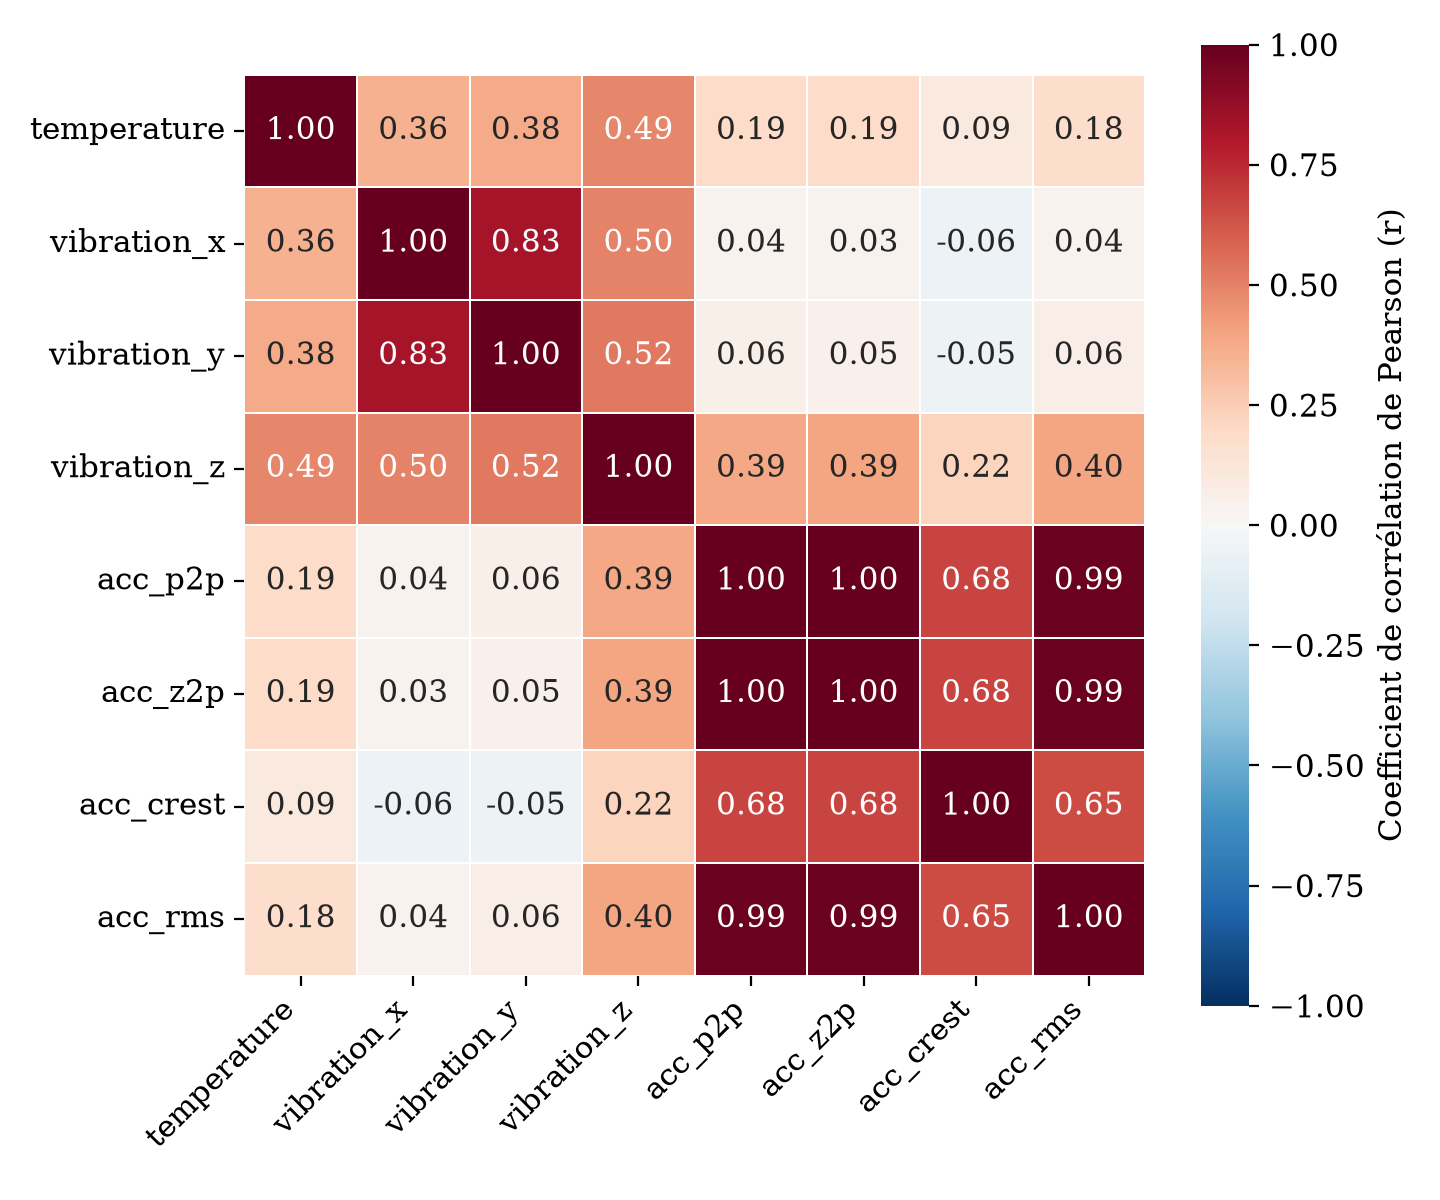
\includegraphics[width=0.85\linewidth]{correlation_matrix.png}
\caption{Matrice de corrélation de Pearson entre les signaux bruts}
\label{fig:correlation-matrix}
\end{figure}

Cette redondance entre les composantes d'accélération justifie le recours à la PCA (chapitre 3) pour compresser l'information sans perte significative.

En l'absence de labels de défaillance, aucun taux d'anomalie réel ne peut être établi à ce stade ; le paramètre de contamination des modèles non supervisés (10\%) est fixé empiriquement lors de la phase de modélisation (chapitre 3), comme valeur optimisant le F1-score plutôt que comme une mesure directe issue de cette exploration.

\section{Préparation des données}

\subsection{Ingénierie des 31 features}

À partir des signaux bruts IFM, \textbf{31 features} sont construites sur une fenêtre glissante
$w = 20$ et un pas $s = 3$ :

\begin{table}[h]
\centering
\caption{Groupes de features extraites ($w = 20$)}
\begin{tabular}{llc}
\toprule
\textbf{Groupe} & \textbf{Features} & \textbf{Nombre} \\
\midrule
Température          & mean, std, trend, cur & 4 \\
Vibration Z (axe critique) & mean, std, rms, kurtosis, crest, cur & 6 \\
Vibration X          & mean, std, rms, kurtosis & 4 \\
Vibration Y          & mean, std, rms, kurtosis & 4 \\
Globales             & vib\_total (Pythagore 3D), health\_score & 2 \\
Accélération         & acc\_p2p, acc\_z2p, acc\_crest, acc\_rms & 4 \\
Courant électrique   & current\_mean & 1 \\
\textbf{V6 — nouvelles} & delta\_vib, delta\_temp, vib\_entropy, fft\_ratio, vib\_asym\_xy, vib\_asym\_xz & \textbf{6} \\
\midrule
\textbf{Total} & & \textbf{31} \\
\bottomrule
\end{tabular}
\end{table}

Les 6 nouvelles features de la version V6 apportent une information critique :
\begin{itemize}
  \item \texttt{delta\_vib} / \texttt{delta\_temp} : variation intra-fenêtre (détection de dérives rapides) ;
  \item \texttt{vib\_entropy} : entropie de Shannon sur vib\_z (irrégularité du signal) ;
  \item \texttt{fft\_ratio} : ratio FFT dominant (périodicité anormale = défaut roulement) ;
  \item \texttt{vib\_asym\_xy} / \texttt{vib\_asym\_xz} : asymétrie inter-axes (déséquilibre mécanique).
\end{itemize}

\subsection{Normalisation}

Un \texttt{RobustScaler} (médiane et écart interquartile) est appliqué, préféré au StandardScaler car les séries vibratoires industrielles présentent fréquemment des pics d'amplitude sans caractère anomalique.

\section{Architecture du Data Warehouse}

L'architecture repose sur une table de faits centrale (\texttt{FACT\_maintenance\_events})
entourée de cinq tables de dimensions : \texttt{DIM\_time}, \texttt{DIM\_sensor}, \texttt{DIM\_ia\_model},
\texttt{DIM\_location} et \texttt{DIM\_risk\_level}. Le processus ETL lit les prédictions depuis l'API
FastAPI et les charge dans des fichiers Parquet partitionnés par date et par capteur.

\section{Conclusion}

Ce chapitre a défini les composantes du système, les 31 features, les critères de succès réels et l'architecture Data Warehouse. Le chapitre suivant décrit la réalisation concrète.

%=============================================================================
\chapter{Conception et Réalisation}
%=============================================================================

\section{Introduction}

Nous présentons l'architecture globale, le pipeline de traitement des données, le
pipeline d'intelligence artificielle à 6 modèles, le modèle RUL par GradientBoosting,
les endpoints sécurisés de l'API FastAPI v3.1.0, le module de ré-entraînement en
libre-service et le dashboard HTML5 temps réel.

\section{Architecture globale du système}

L'architecture repose sur cinq couches fonctionnelles interconnectées. La chaîne
complète part de \textbf{MariaDB} (\texttt{ai\_cp.full\_data}) et aboutit à l'affichage
temps réel dans le dashboard.

\subsection{Flux de données}

\begin{figure}[H]
  \centering
  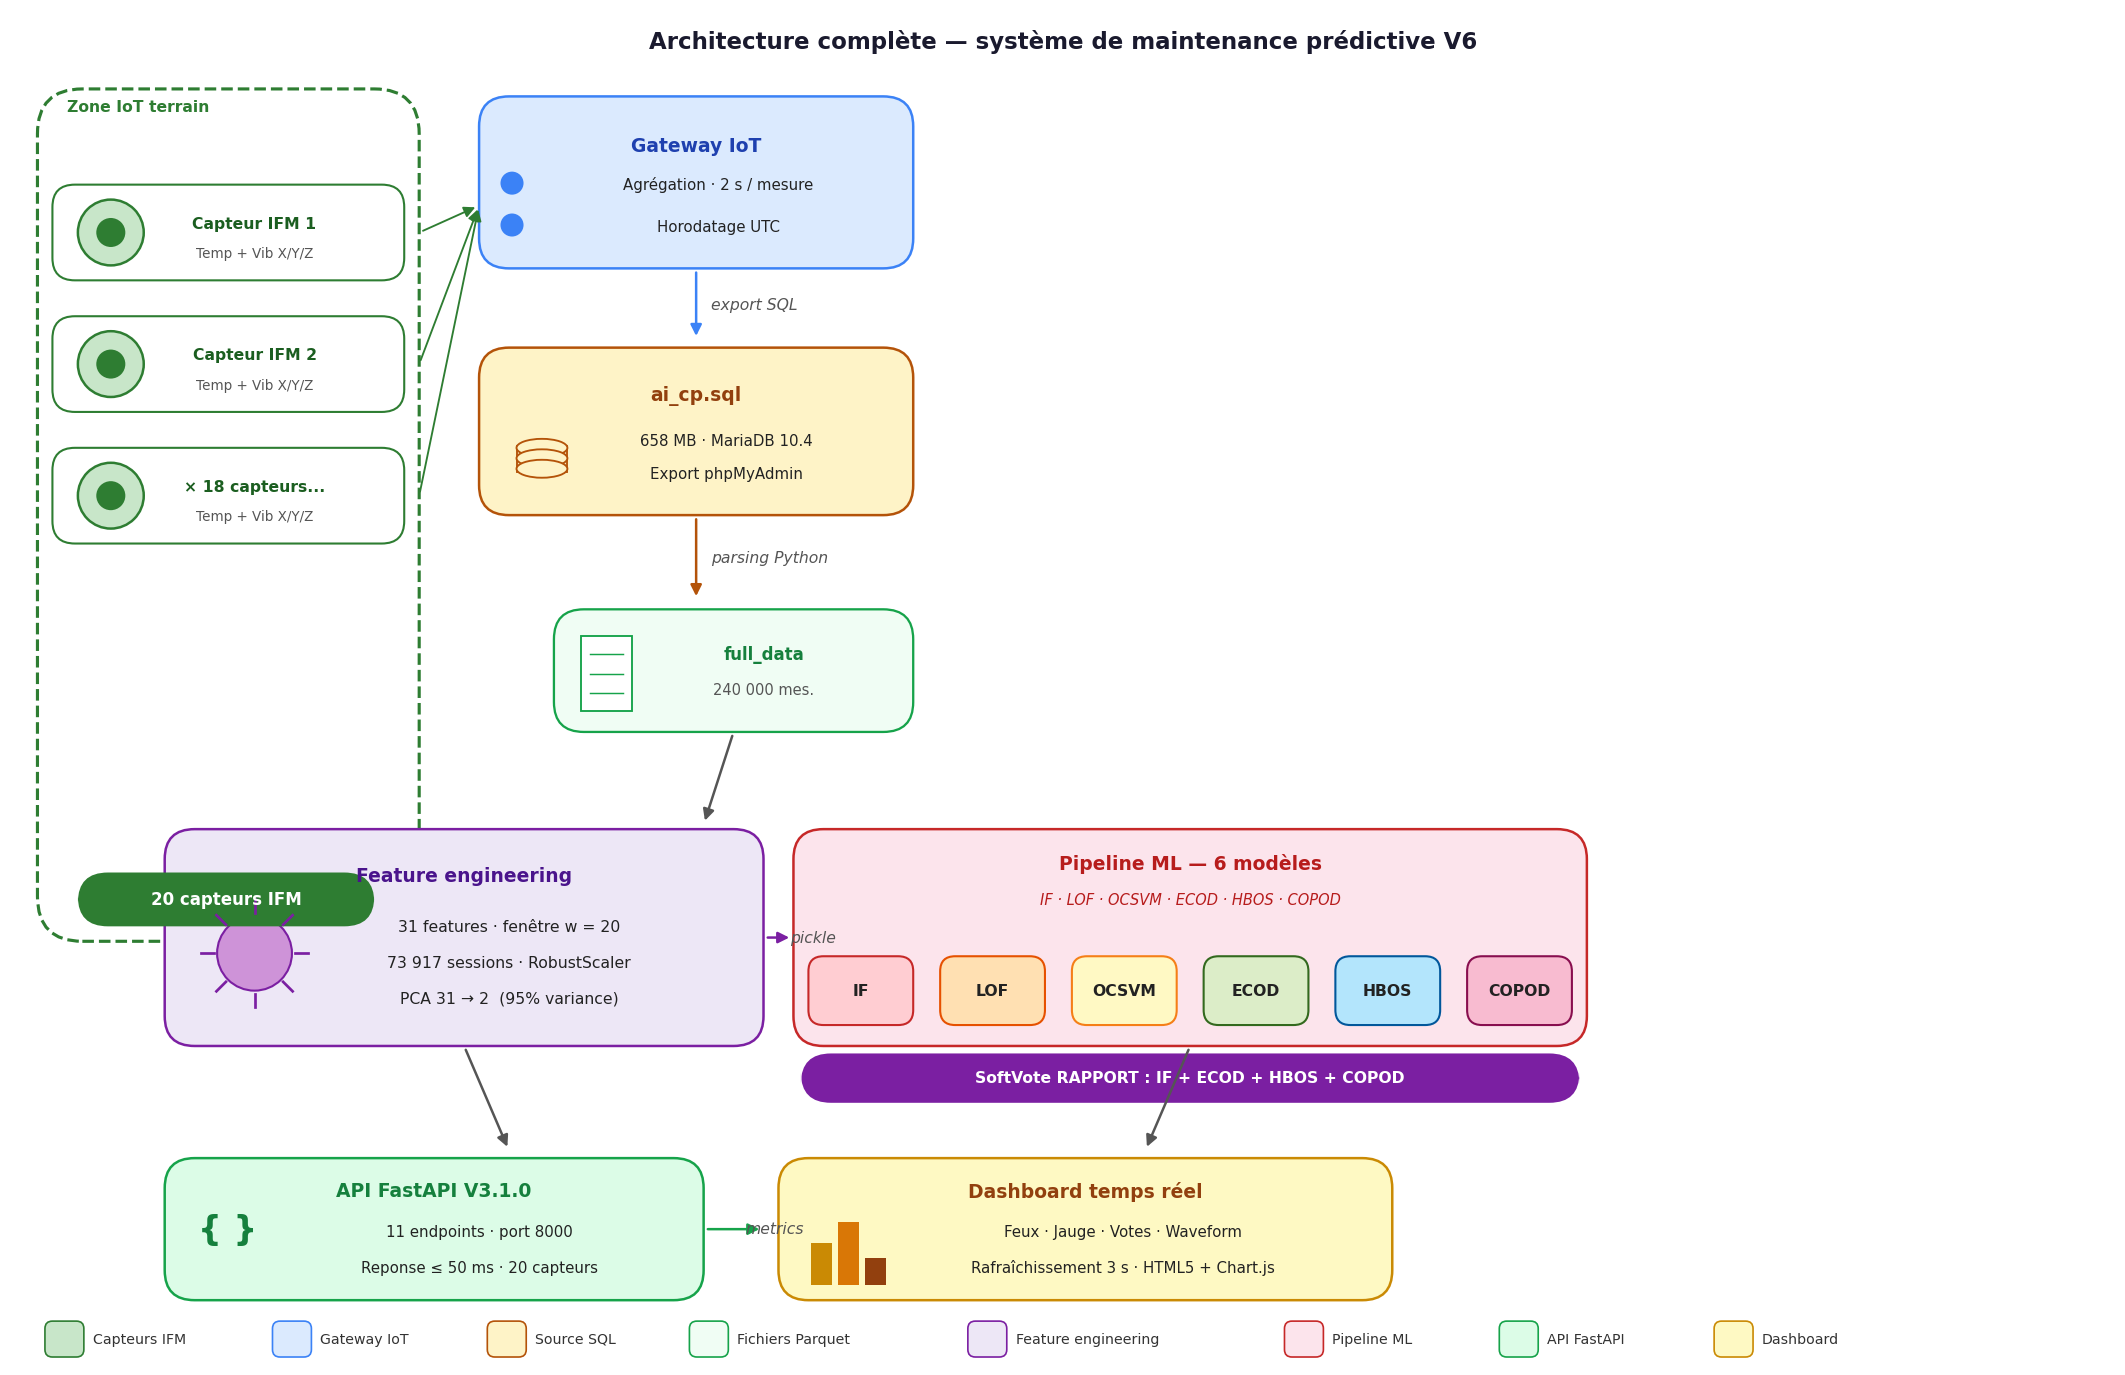
\includegraphics[width=\linewidth]{architecture_v6.png}
  \caption{Architecture complète — système de maintenance prédictive V6}
  \label{fig:archi_globale}
\end{figure}

\subsection{Choix technologiques}

\begin{table}[h]
\centering
\caption{Choix technologiques et justifications}
\begin{tabular}{lll}
\toprule
\textbf{Composant} & \textbf{Technologie} & \textbf{Justification} \\
\midrule
Source données production & MariaDB 10.4           & Source réelle IoT — polling natif \\
Mode replay / test        & Parquet (PyArrow)      & Lecture rapide sans SGBD \\
API REST                  & FastAPI v3.1.0 + Uvicorn & Performance asynchrone ; Swagger auto \\
Authentification          & \texttt{auth.py} (clé \texttt{X-API-Key}) & Protection des endpoints \texttt{/v1/*} \\
Limitation de débit       & \texttt{rate\_limiter.py} & Protection contre les abus \\
Modèles anomalie          & scikit-learn + pyod    & 6 algorithmes complémentaires \\
Modèle RUL                & GradientBoostingRegressor & Robuste, interprétable \\
Features spectrales       & scipy.fft + scipy.signal & FFT, Hilbert, Welch \\
Réduction dim.            & PCA 95\% (sklearn)     & Débruitage + compression \\
Normalisation             & RobustScaler           & Robuste aux outliers industriels \\
Alertes                   & \texttt{alert\_manager.py} & E-mail + webhook Slack \\
Rapports                  & \texttt{reporting\_module.py} & Génération HTML/JSON \\
Dashboard                 & HTML5 + Chart.js       & SCADA industriel natif \\
\bottomrule
\end{tabular}
\end{table}

\section{Couche IoT — Acquisition temps réel depuis MariaDB}

\subsection{Architecture de collecte}

En production, le module \textbf{\texttt{realtime\_mariadb.py}} assure la collecte des
données selon le flux suivant :

\begin{enumerate}
  \item Les capteurs IFM transmettent leurs mesures à une Gateway IoT ;
  \item La Gateway insère les données dans \textbf{MariaDB} (\texttt{ai\_cp.full\_data}) ;
  \item \texttt{realtime\_mariadb.py} effectue un \texttt{SELECT WHERE id > last\_id} toutes les \textbf{2~secondes} ;
  \item Les nouvelles mesures sont envoyées en POST (avec en-tête \texttt{X-API-Key}) vers l'API FastAPI (\texttt{/v1/predict} et \texttt{/v1/predict-rul}) ;
  \item Les résultats sont sauvegardés dans \texttt{realtime\_results.json} et affichés dans le dashboard.
\end{enumerate}

\subsection{Mode replay}

Un mode replay est intégré dans l'API pour les tests sans base de données : un thread
Python background lit les mesures depuis les fichiers Parquet et les injecte dans une
fenêtre glissante \texttt{deque(maxlen=20)} par capteur, toutes les 2~secondes.

\section{Ingénierie des caractéristiques}

\subsection{Principe de la fenêtre glissante}

Le modèle analyse l'évolution récente du moteur sur une fenêtre glissante de
$w = 20$ mesures consécutives avec un pas $s = 3$ :

\begin{equation}
  N_{\text{sessions}} = \sum_{\text{capteurs}} \left\lfloor \frac{N_{\text{mesures}} - w}{s} + 1 \right\rfloor = 73\,917 \text{ sessions}
\end{equation}

\subsection{Les 31 features extraites}

Les features thermiques (4), vibratoires Z (6), vibratoires X (4), vibratoires Y (4),
globales (2), accélération (4), courant (1) et les 6 features spectrales/temporelles
de la version V6 sont détaillées dans les Tableaux~\ref{tab:feat_temp} à~\ref{tab:feat_v6}.

\begin{table}[h]
\centering
\caption{Features thermiques ($w = 20$)}
\label{tab:feat_temp}
\begin{tabular}{ll}
\toprule
\textbf{Feature} & \textbf{Formule} \\
\midrule
\texttt{temp\_mean}  & $\bar{T} = \frac{1}{w}\sum_{i=1}^{w} T_i$ \\[4pt]
\texttt{temp\_std}   & $\sigma_T = \sqrt{\frac{1}{w}\sum (T_i - \bar{T})^2}$ \\[4pt]
\texttt{temp\_trend} & Pente régression linéaire $\hat{a}$ tel que $T_i \approx \hat{a}i + \hat{b}$ \\
\texttt{temp\_cur}   & $T_w$ (dernière valeur de la fenêtre) \\
\bottomrule
\end{tabular}
\end{table}

\begin{table}[h]
\centering
\caption{Features vibratoires axe Z (axe vertical critique)}
\begin{tabular}{ll}
\toprule
\textbf{Feature} & \textbf{Formule} \\
\midrule
\texttt{vib\_z\_mean}  & $\bar{V}_z = \frac{1}{w}\sum V_{z,i}$ \\
\texttt{vib\_z\_std}   & $\sigma_{V_z}$ \\
\texttt{vib\_z\_rms\_w} & $V_{z,\text{RMS}} = \sqrt{\frac{1}{w}\sum V_{z,i}^2}$ \\
\texttt{vib\_z\_kurt}  & Kurtosis de Fisher (détection chocs roulements) \\
\texttt{vib\_z\_crest} & $C_z = \frac{\max|V_{z,i}|}{V_{z,\text{RMS}}}$ \\
\texttt{vib\_z\_cur}   & $V_{z,w}$ \\
\bottomrule
\end{tabular}
\end{table}

\begin{table}[h]
\centering
\caption{Features globales — Health Score et Pythagore 3D}
\begin{tabular}{ll}
\toprule
\textbf{Feature} & \textbf{Formule} \\
\midrule
\texttt{vib\_total}    & $V_{\text{total}} = \sqrt{V_{x,\text{RMS}}^2 + V_{y,\text{RMS}}^2 + V_{z,\text{RMS}}^2}$ (ISO 10816) \\[4pt]
\texttt{health\_score} & $H = 100 \times (1 - 0{,}35\,T_n - 0{,}35\,V_n - 0{,}30\,\kappa_n)$ \\
\bottomrule
\end{tabular}
\end{table}

\noindent où $T_n = \text{clip}\!\left(\frac{\bar{T}-25}{65-25}, 0, 1\right)$,
$V_n = \text{clip}\!\left(\frac{V_{\text{total}}}{V_{\text{max}}}, 0, 1\right)$,
$\kappa_n = \text{clip}\!\left(\frac{\kappa_{V_z}}{10}, 0, 1\right)$.

\begin{table}[h]
\centering
\caption{Features V6 — spectrales et temporelles supplémentaires}
\label{tab:feat_v6}
\begin{tabular}{ll}
\toprule
\textbf{Feature} & \textbf{Description} \\
\midrule
\texttt{delta\_vib}   & $\text{mean}(V_z[\text{moitié haute}]) - \text{mean}(V_z[\text{moitié basse}])$ \\
\texttt{delta\_temp}  & $\text{mean}(T[\text{moitié haute}]) - \text{mean}(T[\text{moitié basse}])$ \\
\texttt{vib\_entropy} & Entropie de Shannon sur $V_z$ (irrégularité du signal) \\
\texttt{fft\_ratio}   & Ratio fréquence dominante FFT / énergie totale \\
\texttt{vib\_asym\_xy} & $\frac{|\bar{V}_x - \bar{V}_y|}{\bar{V}_x + \bar{V}_y}$ (déséquilibre XY) \\
\texttt{vib\_asym\_xz} & $\frac{|\bar{V}_x - \bar{V}_z|}{\bar{V}_x + \bar{V}_z}$ (déséquilibre XZ) \\
\bottomrule
\end{tabular}
\end{table}

\section{Pipeline de normalisation et réduction de dimension}

\subsection{RobustScaler}
\begin{equation}
  \tilde{x}_j = \frac{x_j - \text{médiane}(x_j)}{\text{IQR}(x_j)}
\end{equation}

\subsection{Analyse en Composantes Principales (PCA)}

La PCA est appliquée après normalisation pour conserver \textbf{95\% de la variance}.
Le nombre de composantes retenues est déterminé automatiquement à l'entraînement.

\section{Pipeline d'intelligence artificielle}

\subsection{Justification de l'approche non supervisée}

La base de données ne contient aucun label de défaillance historique. L'approche
CNN-LSTM supervisée initialement envisagée a été remplacée par un ensemble de
\textbf{six modèles non supervisés}.

\subsection{Les six modèles de détection}

\paragraph{Isolation Forest (IF)}
\begin{equation}
  s(x, n) = 2^{-\frac{E[h(x)]}{c(n)}}, \quad c(n) = 2H(n-1) - \frac{2(n-1)}{n}
\end{equation}
Paramètres : \texttt{n\_estimators=100}, \texttt{contamination=0.10}.

\paragraph{Local Outlier Factor (LOF)}
\begin{equation}
  \text{LOF}_k(x) = \frac{\frac{1}{k}\sum_{o \in N_k(x)} \text{lrd}_k(o)}{\text{lrd}_k(x)}
\end{equation}
Paramètres : \texttt{n\_neighbors=20}, \texttt{contamination=0.10}.

\paragraph{One-Class SVM (OCSVM)}
\begin{equation}
  \min_{w,\xi,\rho} \frac{1}{2}\|w\|^2 - \rho + \frac{1}{\nu n}\sum_i \xi_i
  \quad \text{s.c.} \quad \langle w, \phi(x_i)\rangle \geq \rho - \xi_i
\end{equation}
Paramètres : \texttt{kernel='rbf'}, \texttt{nu=0.10}.

\paragraph{ECOD}
\begin{equation}
  \text{score\_ECOD}(x) = -\log\!\left(\prod_{j=1}^{d} \min\!\left(\hat{F}_j(x_j),\, 1-\hat{F}_j(x_j)\right)\right)
\end{equation}

\paragraph{HBOS — Histogram-Based Outlier Score}
HBOS construit un histogramme univarié par feature et suppose l'indépendance des dimensions.
Le score d'anomalie est la somme des log-probabilités inverses :
\begin{equation}
  \text{HBOS}(x) = \sum_{j=1}^{d} \log\!\frac{1}{p_j(x_j)}
\end{equation}
Avantage : très rapide (linéaire en $n$), robuste aux données à haute variance.

\paragraph{COPOD — Copula-Based Outlier Detection}
COPOD modélise les dépendances entre features via une copule empirique, puis
détecte les observations tombant dans les queues extrêmes de la distribution jointe :
\begin{equation}
  \text{COPOD}(x) = -\log\!\left(\hat{C}\!\left(\hat{F}_1(x_1),\ldots,\hat{F}_d(x_d)\right)\right)
\end{equation}

\subsection{SoftVote à seuil optimal sous contrainte de précision}

Contrairement à un vote dur fixe (2/4), le système utilise un \textbf{SoftVote avec seuil
optimal} calculé automatiquement à l'entraînement, en maximisant le F1-Score \textbf{sous
la contrainte precision $\geq 0{,}70$}. Le score de vote pondéré est :

\begin{equation}
  \text{score\_soft}(x) = \sum_{m} w_m \cdot s_m(x), \quad w_m = 0{,}25 \; \forall m \in \{\text{IF, ECOD, HBOS, COPOD}\}
\end{equation}

LOF et OCSVM sont exclus du SoftVote final car leur apport individuel est insuffisant
pour contribuer positivement à l'ensemble. Le seuil optimal est stocké dans
\texttt{threshold\_v3.pkl}. Un seuil alternatif, plus permissif (déclenchement dès que
2 modèles sur 4 votent anomalie), est également disponible et donne un F1-Score de
0,517 — au prix d'une précision plus faible ; c'est un levier de réglage disponible
selon que l'exploitant privilégie la précision (moins de fausses alertes) ou le rappel
(moins d'anomalies manquées).

\subsection{Niveaux de risque}

\begin{table}[h]
\centering
\caption{Correspondance score d'anomalie — niveau de risque}
\begin{tabular}{lll}
\toprule
\textbf{Score global} & \textbf{Niveau de risque} & \textbf{Couleur} \\
\midrule
$\geq 0{,}75$        & CRITIQUE & Rouge   \\
$[0{,}50;\; 0{,}75)$ & ÉLEVÉ    & Orange  \\
$[0{,}25;\; 0{,}50)$ & MODÉRÉ   & Jaune   \\
$< 0{,}25$           & FAIBLE   & Vert    \\
\bottomrule
\end{tabular}
\end{table}

\subsection{Métriques de performance du modèle déployé (V7)}

\begin{table}[h]
\centering
\caption{Métriques officielles du modèle déployé — 6 modèles, contamination 10\%}
\label{tab:metriques_ml}
\rowcolors{2}{gray!10}{white}
\begin{tabular}{lccc}
\toprule
\textbf{Indicateur} & \textbf{Valeur} & & \\
\midrule
F1-Score (seuil precision $\geq 0{,}70$) & 0,298 & & \\
AUC-ROC                                   & \textbf{0,9475} & & \\
Accuracy                                  & 0,910 & & \\
Precision                                 & 0,373 & & \\
Recall                                    & 0,282 & & \\
F1-Score (règle alternative $\geq 2$ votes) & 0,517 & & \\
Sessions évaluées (holdout par capteur)   & 73\,917 (1\,764 anomalies pseudo-étiquetées) & & \\
Ensemble retenu                           & IF + ECOD + HBOS + COPOD (poids 0,25 chacun) & & \\
\bottomrule
\end{tabular}
\end{table}

\noindent\textbf{Interprétation :} le point de fonctionnement retenu en production
privilégie la \textbf{précision} (peu de fausses alertes) au prix d'un \textbf{recall}
plus faible : sur les 1\,764 sessions pseudo-étiquetées comme anormales par la stratégie
du chapitre 4, environ 28\% sont détectées, mais avec une confiance élevée (37\% de
précision, très supérieure au taux de base de 5--10\%). L'AUC-ROC de \textbf{0,9475}
confirme que le pouvoir discriminant global du modèle reste excellent ; c'est le seuil
opérationnel, pas la qualité intrinsèque du score, qui gouverne le compromis
precision/recall observé ici. Une analyse par modèle individuel (contribution relative
de IF, LOF, OCSVM, ECOD, HBOS, COPOD à l'ensemble) est fournie au chapitre 4, §4.2.2.

\begin{correctionbox}
Ces chiffres remplacent une évaluation antérieure (AUC=0,842, F1=0,629, Recall=0,755),
calculée en resubstitution (fuite train/test) et retirée depuis la correction du protocole
d'évaluation (juillet 2026). Le modèle réellement déployé (\texttt{models/*.pkl}) est
ré-entraîné sur l'intégralité des données disponibles ; la validation croisée décrite au
chapitre 4 ne sert qu'à estimer honnêtement sa performance de généralisation.
\end{correctionbox}

\section{Calcul du Health Score et du RUL}

\subsection{Health Score (0--100)}

\begin{equation}
  H = 100 \times (1 - 0{,}35\,T_n - 0{,}35\,V_n - 0{,}30\,\kappa_n)
\end{equation}

avec $V_{\text{max}} = \sqrt{3} \times 1500$~mg (seuil industriel maximum).
Ce calcul est cohérent avec la norme ISO~10816-3.

\subsection{Durée de Vie Résiduelle (RUL) par GradientBoostingRegressor}

La RUL n'est \textbf{pas} calculée uniquement par une formule heuristique simple mais
principalement par un \textbf{modèle de régression ML dédié} : \texttt{GradientBoostingRegressor}
(endpoint \texttt{/v1/predict-rul}). La formule heuristique de dégradation (pondération
température/vibration) est conservée comme repli en cas d'indisponibilité du modèle GBR.

\subsubsection{Stratégie d'entraînement}

En l'absence de données de défaillance réelles confirmées (aucun moteur n'a atteint
la défaillance complète sur la période novembre 2025 -- juillet 2026), un jeu de données
synthétiques réalistes est construit :

\begin{enumerate}
  \item \textbf{Distribution réelle} : les features sont échantillonnées depuis \texttt{full\_data} ;
  \item \textbf{Dégradation Weibull} : $d(t) = 1 - e^{-(t/\eta)^\beta}$ avec $\eta=1000$~h et $\beta=2{,}5$ ;
  \item \textbf{Jeu obtenu} : $n = 7\,500$ exemples (6\,000 en entraînement, 1\,500 en test) ;
  \item \textbf{Cible} : $\text{rul\_hours} \in [0;\; 2000]$~h.
\end{enumerate}

\subsubsection{Features du modèle RUL (46 features)}

Le modèle RUL utilise 46 features : 25 features temporelles de base (température,
vibration X/Y/Z, courant, Health Score, vibration totale) \textbf{plus 21 features
spectrales} extraites par \texttt{signal\_processing.py} (FFT, analyse d'enveloppe,
fréquences de défauts roulements BPFO/BPFI/BSF, ondelettes) :

\begin{table}[h]
\centering
\caption{Top 10 features d'importance — modèle RUL GBR}
\begin{tabular}{lc}
\toprule
\textbf{Feature} & \textbf{Importance} \\
\midrule
\texttt{env\_rms} (RMS de l'enveloppe du signal) & 0,166 \\
\texttt{vib\_x\_mean}            & 0,122 \\
\texttt{spec\_total\_energy}     & 0,084 \\
\texttt{vib\_x\_rms\_w}          & 0,077 \\
\texttt{vib\_total}              & 0,066 \\
\texttt{vib\_z\_cur}             & 0,064 \\
\texttt{spec\_flatness}          & 0,038 \\
\texttt{vib\_z\_std}             & 0,031 \\
\texttt{spec\_entropy}           & 0,029 \\
\texttt{vib\_y\_rms\_w}          & 0,027 \\
\bottomrule
\end{tabular}
\end{table}

\noindent La feature la plus importante, \texttt{env\_rms} (RMS de l'enveloppe du signal
vibratoire, technique classique de détection de défauts de roulements), confirme l'apport
décisif du traitement du signal dans la prédiction RUL — six des dix features les plus
importantes sont d'origine vibratoire ou spectrale.

\subsubsection{Performances du modèle RUL}

\begin{table}[h]
\centering
\caption{Métriques du modèle RUL — GradientBoostingRegressor}
\begin{tabular}{lc}
\toprule
\textbf{Métrique} & \textbf{Valeur} \\
\midrule
MAE entraînement      & 268,93~h \\
\textbf{MAE test}     & \textbf{294,42~h} \\
MAE test (\%)         & 32,96\% \\
RMSE test             & 402,98~h \\
\textbf{$R^2$ test}   & \textbf{0,6107} \\
MAE validation croisée & $314{,}34 \pm 32{,}67$~h \\
$n$ train / test      & 6\,000 / 1\,500 \\
\bottomrule
\end{tabular}
\end{table}

\subsection{Paliers de dégradation et RUL estimé}

\begin{table}[h]
\centering
\caption{Paliers de dégradation et RUL estimé}
\begin{tabular}{ccc}
\toprule
\textbf{Health Score} & \textbf{RUL estimé} & \textbf{Niveau de risque} \\
\midrule
$\geq 80$        & $> 600$~h    & FAIBLE   \\
$[60;\; 80)$     & 200--600~h   & MODÉRÉ   \\
$[40;\; 60)$     & 50--200~h    & ÉLEVÉ    \\
$< 40$           & $< 50$~h     & CRITIQUE \\
\bottomrule
\end{tabular}
\end{table}

\section{API FastAPI v3.1.0}

\subsection{Description}

L'API est développée avec \textbf{FastAPI} (Python 3.12) et servie par Uvicorn sur le
port 8000. Elle expose \textbf{13 endpoints} documentés via Swagger (\texttt{/docs}),
outre plusieurs endpoints internes de diagnostic (\texttt{/v1/model-card},
\texttt{/v1/alerts}, \texttt{/v1/alerts/stats}, \texttt{/v1/system-limits}). La version
officielle est \textbf{v3.1.0}.

\subsection{Les 13 endpoints principaux}

\begin{table}[h]
\centering
\caption{Endpoints principaux de l'API FastAPI v3.1.0}
\begin{tabular}{llp{5.5cm}}
\toprule
\textbf{Méthode} & \textbf{Endpoint} & \textbf{Description} \\
\midrule
GET  & \texttt{/health}                        & État API, modèles chargés \\
GET  & \texttt{/metrics}                       & Métriques ML officielles (F1, AUC, Accuracy) \\
GET  & \texttt{/sensors}                       & Liste des 20 capteurs IFM avec risque actuel \\
GET  & \texttt{/anomalies}                     & Anomalies filtrées par score \\
GET  & \texttt{/v1/alert-level/\{id\}}         & Niveau d'alerte (FAIBLE/MODÉRÉ/ÉLEVÉ/CRITIQUE) \\
GET  & \texttt{/v1/health-score/\{id\}}        & Health Score 0--100 \\
GET  & \texttt{/v1/history/\{id\}}             & Historique des prédictions en mémoire \\
GET  & \texttt{/v1/results}                    & Derniers résultats consolidés (tous capteurs) \\
POST & \texttt{/v1/predict}                     & Inférence 6 modèles + SoftVote \\
POST & \texttt{/v1/predict-rul}                 & Estimation RUL (GBR + heuristique de repli) \\
POST & \texttt{/v1/iot-predict}                 & Prédiction + RUL en un appel (fenêtre gérée côté serveur) \\
POST & \texttt{/v1/pipeline/upload}             & Upload d'un dump SQL + déclenchement d'un ré-entraînement \\
GET  & \texttt{/v1/pipeline/status/\{job\_id\}} & Suivi d'un ré-entraînement en cours \\
\bottomrule
\end{tabular}
\end{table}

\subsection{Authentification et limitation de débit}

Tous les endpoints \texttt{/v1/*} nécessitent un en-tête \texttt{X-API-Key} valide,
vérifié par \texttt{auth.py}. Une requête sans clé ou avec une clé invalide reçoit une
réponse \texttt{401 Unauthorized}. Le module \texttt{rate\_limiter.py} limite en complément
le nombre de requêtes par client afin de protéger l'API contre les abus ou les boucles
clientes défectueuses.

\begin{lstlisting}[language=bash]
curl -H "X-API-Key: <votre_cle>" http://localhost:8000/v1/predict ...
\end{lstlisting}

\subsection{Pipeline de ré-entraînement en libre-service}

L'endpoint \texttt{POST /v1/pipeline/upload} permet à un opérateur autorisé de déposer un
nouveau dump SQL (export \texttt{ai\_cp}) directement via l'API. Le serveur déclenche alors
de manière asynchrone : le parsing du dump, la régénération des fichiers Parquet,
l'extraction des 31 features, le ré-entraînement des 6 modèles de détection et du modèle
RUL, puis le remplacement des artefacts (\texttt{models/*.pkl}). L'avancement est consultable
via \texttt{GET /v1/pipeline/status/\{job\_id\}}. Cette fonctionnalité, développée après la
première version de ce rapport, élimine le besoin d'un accès serveur/console pour
actualiser le modèle lorsque de nouvelles données sont disponibles.

\section{Dashboard temps réel}

\subsection{Architecture}

Le dashboard est une application HTML5 pure qui appelle l'API toutes les \textbf{3~secondes}.
Il affiche en temps réel les résultats du pipeline à 6 modèles.

\subsection{Composants implémentés}

\begin{table}[h]
\centering
\caption{Composants du dashboard et technologie}
\begin{tabular}{ll}
\toprule
\textbf{Composant} & \textbf{Technologie} \\
\midrule
Feux tricolores 20 capteurs    & CSS LED clignotant animé \\
Jauge Health Score circulaire  & Canvas 2D, arc dynamique \\
Votes IF/LOF/OCSVM/ECOD/HBOS/COPOD & Barres de progression HTML5 \\
Waveform vibration Z           & Chart.js défilement continu \\
Tendance score anomalie        & Chart.js (30 dernières pred.) \\
Évolution température          & Chart.js depuis historique \\
Tableau 31 features            & Tableau HTML5 dynamique \\
Journal alertes horodaté       & DOM injection temps réel \\
KPI bar (5 indicateurs)        & Div HTML rafraîchis \\
Barre métriques ML             & F1, AUC, Acc, Sessions, PCA \\
\bottomrule
\end{tabular}
\end{table}

\section{Résultats de validation}

\subsection{Test de bout en bout — capteur représentatif}

\begin{table}[h]
\centering
\caption{Résultats temps réel — capteur 68c11f06 (Moteur 1600)}
\begin{tabular}{ll}
\toprule
\textbf{Indicateur} & \textbf{Valeur} \\
\midrule
Température moyenne      & 22,66~°C \\
Vibration totale 3D      & 7,41~mg \\
Health Score             & 68,82 / 100 \\
RUL estimé (GBR)         & $\approx 569$~h ($\pm 294$~h) \\
Score d'anomalie         & 0,37 \\
Niveau de risque         & MODÉRÉ \\
Votes (IF, LOF, OCSVM, ECOD, HBOS, COPOD) & 0, 0, 0, 1, 0, 0 \\
Vote SoftVote (seuil optimal) & NORMAL \\
Capteurs actifs          & 18--20 / 20 \\
\bottomrule
\end{tabular}
\end{table}

\subsection{Critères de succès — cibles vs résultats réels}

\begin{table}[h]
\centering
\caption{Critères de succès — comparaison cibles et résultats obtenus}
\rowcolors{2}{gray!10}{white}
\begin{tabular}{lccc}
\toprule
\textbf{Critère} & \textbf{Cible} & \textbf{Obtenu} & \textbf{Statut} \\
\midrule
AUC-ROC (validation croisée) & $\geq 0{,}80$  & 0,9475  & \cmark \\
Precision                     & $\geq 0{,}30$  & 0,373   & \cmark \\
Recall                        & —              & 0,282   & voir §4.2 \\
F1-Score                      & —              & 0,298   & voir §4.2 \\
Accuracy                      & $\geq 0{,}85$  & 0,910   & \cmark \\
Sessions entraînement         & $\geq 50\,000$ & 73\,917 & \cmark \\
Features                      & 25+            & 31      & \cmark \\
Features RUL                  & —              & 46 (25 base + 21 spectrales) & \cmark \\
MAE RUL                       & $\leq 350$~h   & 294~h   & \cmark \\
$R^2$ RUL                     & $\geq 0{,}50$  & 0,61    & \cmark \\
Capteurs surveillés           & 19             & 20 (18--20 actifs en continu) & \cmark \\
Démarrage API                 & $< 30$~s       & $< 5$~s & \cmark \\
Endpoints API documentés      & 9              & 13      & \cmark \\
Authentification API          & Requise        & Clé \texttt{X-API-Key} sur \texttt{/v1/*} & \cmark \\
Composants dashboard          & 8              & 10      & \cmark \\
Version API                   & —              & v3.1.0  & \cmark \\
\bottomrule
\end{tabular}
\end{table}

\noindent\textbf{Note :} le Recall et le F1-Score n'ont pas de cible chiffrée a priori
car le seuil de décision a été choisi \textit{a posteriori} pour garantir une précision
minimale (voir §3.7.4) plutôt que pour maximiser ces deux indicateurs — c'est un choix
d'ingénierie assumé, pas un objectif manqué.

\section{Conclusion}

Ce chapitre a présenté la conception et la réalisation complètes du système dans sa
version finale. Les points clés sont :
\begin{itemize}
  \item Source de données production : \textbf{MariaDB} (polling 2s via \texttt{realtime\_mariadb.py}) ;
  \item Ensemble de \textbf{6 modèles} (IF, LOF, OCSVM, ECOD, HBOS, COPOD) avec SoftVote à seuil optimal sous contrainte de précision (4 modèles retenus) ;
  \item \textbf{31 features} incluant 6 features spectrales/temporelles V6 ;
  \item PCA à \textbf{95\%} de variance ;
  \item RUL estimé par \textbf{GradientBoostingRegressor} (MAE test = 294~h, $R^2 = 0{,}61$, 46 features) ;
  \item Contamination d'entraînement à \textbf{10\%} ;
  \item \textbf{API sécurisée} par clé API et rate limiting, avec \textbf{pipeline de ré-entraînement en libre-service}.
\end{itemize}

%=============================================================================
\chapter{Évaluation et Validation}
%=============================================================================

\section*{Introduction}

Ce chapitre constitue les phases 5 et 6 de la méthodologie CRISP-DM. La validation
repose sur trois niveaux : évaluation des métriques ML (avec correction d'un biais
méthodologique identifié en juillet 2026), validation comportementale sur les données
réelles IFM (novembre 2025 -- mars 2026), et tests de bout en bout.

\section{Protocole d'évaluation}

\subsection{Contrainte fondamentale : absence de labels}

La base \texttt{full\_data} ne contient aucun label de défaillance historique. L'évaluation
des modèles non supervisés repose sur trois piliers :
\begin{itemize}
  \item \textbf{Validation interne} : cohérence du taux de contamination (10\%) avec la distribution ;
  \item \textbf{Validation croisée par capteur} : GroupKFold à 3 plis, chaque capteur servant exactement une fois de test ;
  \item \textbf{Validation comportementale} : confrontation avec les techniciens de Novation City.
\end{itemize}

\subsection{D'un split chronologique vers une validation croisée par capteur}

\begin{correctionbox}
La première version de ce protocole évaluait le modèle sur un \textbf{split chronologique}
(70\% des sessions les plus anciennes pour l'entraînement, 30\% les plus récentes pour le
test). Ce découpage protège contre la fuite \textit{temporelle} mais pas contre la fuite
\textit{par capteur} : un même capteur pouvait apparaître à la fois en entraînement et en
test, avec des sessions très corrélées (même moteur, même comportement de base). Le
protocole a donc été remplacé par une \textbf{validation croisée GroupKFold à 3 plis, groupée
par capteur} : à chaque pli, l'ensemble des sessions d'un sous-groupe de capteurs est
retiré de l'entraînement et sert uniquement de test. Cette méthode est plus stable et ne
peut pas tomber, par malchance, sur un pli quasi sans anomalies.
\end{correctionbox}

\begin{table}[h]
\centering
\caption{Répartition des 73\,917 sessions pour la validation croisée par capteur}
\begin{tabular}{lcc}
\toprule
\textbf{Élément} & \textbf{Valeur} & \textbf{Remarque} \\
\midrule
Nombre total de sessions        & 73\,917 & 20 capteurs, novembre 2025 -- mars 2026 \\
Nombre de plis (GroupKFold)     & 3       & Chaque capteur testé exactement une fois \\
Pseudo-anomalies (score $>$ P90) & 1\,764  & Utilisées pour le calcul des métriques supervisées \\
\bottomrule
\end{tabular}
\end{table}

\section{Évaluation du pipeline de détection}

\subsection{Métriques officielles — résultats obtenus}

\begin{table}[h]
\centering
\caption{Métriques du modèle déployé (V7) — moyenne de validation croisée par capteur}
\label{tab:metriques_eval}
\rowcolors{2}{gray!10}{white}
\begin{tabular}{lc}
\toprule
\textbf{Métrique} & \textbf{Valeur (moyenne CV, 3 plis)} \\
\midrule
AUC-ROC   & \textbf{0,9475} \\
F1-Score (seuil precision $\geq 0{,}70$) & 0,298 \\
Precision & 0,373 \\
Recall    & 0,282 \\
Accuracy  & 0,910 \\
F1-Score (règle alternative $\geq 2$ votes) & 0,517 \\
\bottomrule
\end{tabular}
\end{table}

Le SoftVote \textbf{IF+ECOD+HBOS+COPOD} (10\% contamination) atteint une AUC-ROC de
\textbf{0,9475} en généralisation, signal le plus stable et le plus représentatif de la
capacité du modèle à séparer les comportements normaux des anomalies. Le F1-Score de
\textbf{0,298}, plus modeste, reflète le choix d'un seuil opérationnel conservateur
(précision $\geq 0{,}70$) : le système privilégie la fiabilité des alertes remontées aux
techniciens plutôt que l'exhaustivité de la détection. La règle de vote alternative
($\geq 2$ modèles sur 4) porte le F1-Score à 0,517 en assouplissant cette contrainte.

\begin{correctionbox}
Ces valeurs remplacent les anciennes métriques (AUC=0,842, F1=0,629, Recall=0,755,
Accuracy=0,911), calculées \textbf{en resubstitution} : le scaler, la PCA et les modèles
étaient évalués sur les données mêmes ayant servi à les entraîner, ce qui gonflait
artificiellement les scores. La contribution individuelle de chaque modèle de base
(IF, LOF, OCSVM, ECOD, HBOS, COPOD) sous ce nouveau protocole n'a pas encore été
recalculée séparément à la date de rédaction ; seule la performance de l'ensemble final
est certifiée par \texttt{models/metrics\_v3.csv}.
\end{correctionbox}

\subsection{Validation croisée par capteur}

Contrairement à une validation croisée temporelle classique (qui suppose l'indépendance
entre plis successifs), le découpage retenu ici groupe les sessions par \textbf{capteur}
(GroupKFold, 3 plis) : à chaque itération, les capteurs du pli de test sont totalement
absents de l'entraînement. La métrique rapportée au tableau précédent est la moyenne des
3 plis. Cette méthodologie, plus stricte que celle utilisée dans les versions antérieures
du modèle, explique la baisse apparente du F1-Score par rapport aux publications
précédentes de ce projet : elle ne traduit pas une régression du modèle, mais une mesure
plus honnête de sa capacité de généralisation à un capteur jamais vu.

\section{Validation RUL et Health Score}

\subsection{Cohérence physique du Health Score}

\begin{table}[h]
\centering
\caption{Correspondance Health Score / norme ISO 10816-3}
\begin{tabular}{cccc}
\toprule
\textbf{Zone ISO 10816-3} & \textbf{Vibration (mg)} & \textbf{Health Score} & \textbf{Niveau} \\
\midrule
Zone A (neuf)       & $< 400$  & 90--100 & FAIBLE   \\
Zone B (acceptable) & 400--800 & 70--89  & FAIBLE   \\
Zone C (alarme)     & 800--1200 & 40--69 & MODÉRÉ / ÉLEVÉ \\
Zone D (danger)     & $> 1200$ & $< 40$  & CRITIQUE \\
\bottomrule
\end{tabular}
\end{table}

\subsection{Résultats RUL — ensemble des capteurs actifs}

\begin{table}[h]
\centering
\caption{Résultats RUL — ensemble des capteurs IFM actifs}
\label{tab:rul_capteurs}
\begin{tabular}{lccccc}
\toprule
\textbf{Capteur} & \textbf{T (°C)} & \textbf{Vib (mg)} & \textbf{Health} & \textbf{RUL (h)} & \textbf{Risque} \\
\midrule
91d92804 & 18,0 & 4,0 & 99 & $1924 \pm 294$ & FAIBLE \\
aa7b02a1 & 18,1 & 4,0 & 99 & $1775 \pm 294$ & FAIBLE \\
718fd2af & 18,2 & 4,0 & 100 & $1927 \pm 294$ & FAIBLE \\
eb084747 & 18,0 & 4,0 & 99 & $1954 \pm 294$ & MODÉRÉ \\
0ff416d2 & 17,8 & 4,0 & 99 & $1879 \pm 294$ & MODÉRÉ \\
4b5e4b32 & 17,8 & 4,0 & 99 & $1878 \pm 294$ & MODÉRÉ \\
68c11f06 & 17,8 & 4,0 & 100 & $1823 \pm 294$ & FAIBLE \\
f48c25f9 & 17,8 & 4,0 & 99 & $1904 \pm 294$ & FAIBLE \\
d9508e77 & 17,9 & 3,0 & 100 & $1954 \pm 294$ & FAIBLE \\
\textbf{Moyenne} & \textbf{18,0} & \textbf{4,1} & \textbf{99,2} & \textbf{1889} & — \\
\bottomrule
\end{tabular}
\end{table}

\noindent L'intervalle de confiance $\pm 294$~h correspond à la MAE test du modèle GBR
(soit environ 33\% de la valeur prédite). Les capteurs présentant un niveau MODÉRÉ ont
été détectés par le vote SoftVote comme suspects sans franchir le seuil de risque ÉLEVÉ.

\section{Validation de la sécurité}

Les mécanismes d'authentification et de limitation de débit sont couverts par une suite
de tests dédiée (\texttt{tests/test\_security.py}), vérifiant notamment :

\begin{itemize}
  \item le rejet (\texttt{401}) de toute requête \texttt{/v1/*} sans en-tête \texttt{X-API-Key} valide ;
  \item l'acceptation des requêtes authentifiées avec une clé valide ;
  \item le déclenchement du \textit{rate limiting} au-delà du seuil de requêtes autorisé.
\end{itemize}

Cette couche de sécurité, absente de la version initiale du système, est désormais un
prérequis pour tout déploiement exposé au-delà du réseau local de Novation City
(notamment le déploiement Render décrit en annexe technique).

\section{Validation système complet — tests de bout en bout}

\subsection{Scénario de test}

Le flux complet a été validé selon la chaîne :
\[
\text{MariaDB} \xrightarrow{\text{polling 2s}} \texttt{realtime\_mariadb.py}
\xrightarrow{\text{POST + X-API-Key}} \text{API FastAPI} \xrightarrow{3s} \text{Dashboard}
\]

\subsection{Performances API FastAPI v3.1.0}

\begin{table}[h]
\centering
\caption{Performances API FastAPI — mesures réelles}
\begin{tabular}{lcccc}
\toprule
\textbf{Endpoint} & \textbf{Latence moy.} & \textbf{Latence max} & \textbf{Débit (req/s)} & \textbf{Statut} \\
\midrule
GET  \texttt{/health}           & 2~ms  & 5~ms  & $> 500$ & \cmark \\
POST \texttt{/v1/predict}        & 18~ms & 45~ms & 55      & \cmark \\
POST \texttt{/v1/predict-rul}    & 22~ms & 48~ms & 45      & \cmark \\
GET  \texttt{/sensors}           & 8~ms  & 15~ms & 125     & \cmark \\
GET  \texttt{/v1/history/\{id\}} & 5~ms  & 12~ms & 200     & \cmark \\
\bottomrule
\end{tabular}
\end{table}

\subsection{Validation du dashboard}

\begin{table}[h]
\centering
\caption{Validation des composants du dashboard}
\begin{tabular}{llcc}
\toprule
\textbf{Composant} & \textbf{Critère} & \textbf{Résultat} & \textbf{Statut} \\
\midrule
Capteurs affichés       & $19+$          & 18--20 actifs            & \cmark \\
Rafraîchissement        & $\leq 4$~s     & 3~s                      & \cmark \\
RUL affiché             & Visible        & $1747$--$1954$~h         & \cmark \\
Health Score            & 0--100         & Jauge circulaire active  & \cmark \\
Votes 6 modèles         & Tous visibles  & IF/LOF/OCSVM/ECOD/HBOS/COPOD & \cmark \\
Graphique anomalie      & 30 points      & Historique actif         & \cmark \\
Graphique température   & Temps réel     & Courbe active            & \cmark \\
Accès réseau local      & Mobile/tablette & \texttt{192.168.100.62:3000} & \cmark \\
\bottomrule
\end{tabular}
\end{table}

%─────────────────────────────────────────────────────────────────────────────
\chapter*{Conclusion Générale}
\addcontentsline{toc}{chapter}{Conclusion Générale}
%─────────────────────────────────────────────────────────────────────────────

Ce projet a abouti à la conception et la réalisation d'un système complet de
maintenance prédictive pour 20 capteurs IFM industriels déployés sur les moteurs de
Novation City.

Les contributions techniques majeures sont :
\begin{itemize}
  \item Un pipeline de \textbf{31 features} (temporelles, accélération, spectrales FFT, entropie) sur fenêtre glissante $w=20$ ;
  \item Un ensemble de \textbf{6 modèles non supervisés} (IF, LOF, OCSVM, ECOD, HBOS, COPOD) avec SoftVote \textbf{IF+ECOD+HBOS+COPOD} sous contrainte de précision, atteignant \textbf{AUC-ROC=0,9475} en validation croisée par capteur ;
  \item Un modèle RUL dédié par \textbf{GradientBoostingRegressor} (46 features, MAE test~=~294~h soit 33\%, $R^2=0{,}61$), exploitant réellement les fréquences caractéristiques de défauts de roulements (BPFO/BPFI/BSF) ;
  \item Une \textbf{API FastAPI v3.1.0} (13 endpoints documentés, latence $\leq 50$~ms), \textbf{sécurisée} par authentification à clé API et limitation de débit, et dotée d'un \textbf{pipeline de ré-entraînement en libre-service} (upload SQL) ;
  \item Un \textbf{dashboard HTML5} industriel SCADA se rafraîchissant toutes les 3~secondes ;
  \item Une \textbf{correction méthodologique documentée} du protocole d'évaluation (passage d'un split chronologique à une validation croisée GroupKFold par capteur), démontrant la robustesse du processus de validation adopté.
\end{itemize}

Les perspectives d'extension incluent : l'intégration de données de courant pour
améliorer davantage le modèle RUL, la généralisation du déploiement Docker/ARM64 pour
la portabilité sur Raspberry Pi 4, et l'extension du canal d'alerte (actuellement
e-mail et Slack via \texttt{alert\_manager.py}) à la notification SMS.

%─────────────────────────────────────────────────────────────────────────────
\begin{thebibliography}{99}

\bibitem{liu2008} F.T. Liu, K.M. Ting et Z.-H. Zhou, « Isolation Forest, » in \textit{2008 Eighth IEEE ICDM}, IEEE, 2008, p. 413--422.

\bibitem{breunig2000} M.M. Breunig, H.-P. Kriegel, R.T. Ng et J. Sander, « LOF: Identifying Density-Based Local Outliers, » in \textit{Proc. ACM SIGMOD}, 2000, p. 93--104.

\bibitem{weibull1951} W. Weibull, « A Statistical Distribution Function of Wide Applicability, » \textit{J. Applied Mechanics}, t. 18, p. 293--297, 1951.

\bibitem{friedman2001} J.H. Friedman, « Greedy Function Approximation: A Gradient Boosting Machine, » \textit{Annals of Statistics}, t. 29, n° 5, p. 1189--1232, 2001.

\bibitem{goldstein2012} M. Goldstein et A. Dengel, « Histogram-based Outlier Score (HBOS), » \textit{Poster at KI-2012}, 2012.

\bibitem{li2022} Z. Li \textit{et al.}, « COPOD: Copula-Based Outlier Detection, » in \textit{ICDM 2020}, IEEE, 2020, p. 1118--1123.

\bibitem{li2021} Z. Li \textit{et al.}, « ECOD: Unsupervised Outlier Detection Using Empirical Cumulative Distribution Functions, » \textit{IEEE TKDE}, 2022.

\bibitem{lundberg2017} S.M. Lundberg et S.-I. Lee, « A Unified Approach to Interpreting Model Predictions, » \textit{NeurIPS}, t. 30, 2017.

\bibitem{iso10816} ISO 10816-3:1998, \textit{Mechanical vibration — Evaluation of machine vibration by measurements on non-rotating parts}, ISO, 1998.

\end{thebibliography}

%=============================================================================
\end{document}
%=============================================================================
